\documentclass{article}

\usepackage[margin=1in]{geometry} 
\usepackage{amsmath,amsthm,amssymb,amsfonts, fancyhdr, color, comment, graphicx, environ,bbm}
\usepackage[dvipsnames]{xcolor}
\usepackage{subcaption}
\usepackage{mdframed}
\usepackage[shortlabels]{enumitem}
\usepackage{indentfirst}
\usepackage{hyperref}
\usepackage{placeins}
\usepackage{comment} %Comment large blocks
\usepackage{xfrac}
\usepackage{float} % To use "H" to force tables to be where wanted
\usepackage{booktabs} % Makes output from knittr:kable look better
\usepackage{parskip} %No indents for paragraphs
\usepackage[shortlabels]{enumitem} % To enumerate with letters
\hypersetup{
 colorlinks=true,
 linkcolor=blue,
 filecolor=magenta, 
 urlcolor=blue,
}
\pagestyle{fancy}
\usepackage{todonotes}

\newcommand{\E}{\mathbb{E}}
\renewcommand{\H}{\mathcal{H}}
\renewcommand{\L}{\mathcal{L}}
\newcommand{\dU}[1]{\ensuremath\frac{\partial u}{\partial #1}}
\newcommand{\dV}[1]{\ensuremath\frac{\partial v}{\partial #1}}
\newcommand{\ppx}[2]{\ensuremath\frac{\partial #1}{\partial #2}}
\newcommand{\ddx}[2]{\ensuremath\frac{d #1}{d #2}}
\newcommand{\indp}{\perp\!\!\!\perp} 

%\usepackage{mathpazo} %Dylan's fancy math bullshit that I don't want
\usepackage{microtype}
\usepackage{graphicx}
\usepackage{setspace}

%Footnote without a number
\newcommand\blfootnote[1]{%
  \renewcommand\thefootnote{}\footnote{#1}%
  \addtocounter{footnote}{-1}%
}

% Problem formatting [Alex]

\newenvironment{problem}[1]
    { \begin{mdframed}[backgroundcolor=Periwinkle!20] \textbf{(#1)} }
    {  \end{mdframed}}
% Define solution environment
\newenvironment{solution}{\textbf{Solution}\\}

%%%%%%%%%%%%%%%%%%%%%%%%%%%%%%%%%%%%%%%%%%%%%
%Fill in the appropriate information below
\lhead{Problem Set 1}
\rhead{Empirical Analysis} 
\title{Problem Set 1}
\author{Alex Weinberg \and Isaac Norwich \and Jose M. Quintero}

%%%%%%%%%%%%%%%%%%%%%%%%%%%%%%%%%%%%%%%%%%%%%
\begin{document}
\maketitle

Our code can be found in this GitHub respository: \url{https://github.com/jmquintero925/Metrics-III/tree/main/ps1Heckman}


%%%%%%%%%%%%%%%%%%%%%%%%%%%%%%%%%% QUESTION 1 %%%%%%%%%%%%%%%%%%%%%%%%%%%%%%%%%
\section*{Problem 1}
Comment on Richard Feynman’s commentary on social science and John Geweke’s further claim that most empirical papers in economics are wrong.
\begin{problem}{a}
What are the rewards to the author for doing careful empirical research?
\end{problem}
\begin{problem}{b}
Should empirical economic analysts be required to submit pre-analysis
plans before conducting research?
\end{problem}
\begin{problem}{c}
Explain how Bayesian, likelihood, and classical statistical inference approaches differ in learning from data.
\end{problem}
\begin{problem}{d}
 Read the papers by Christensen and Miguel (2018) and Chang and Li (2015). In light of results reported in these papers, is Feynman right? Is economics a pseudoscience?
\end{problem}


\newpage
%%%%%%%%%%%%%%%%%%%%%%%%%%%%%%%%%% QUESTION 3 %%%%%%%%%%%%%%%%%%%%%%%%%%%%%%%%%
\section*{Problem 2}
What is the “credibility approach” in economics? See, e.g., the Angrist
(2022) and Card (2022) Nobel lectures, as well as Hull et al. (2022)
\begin{problem}{a}
How is credibility defined? What are its ingredients?
\end{problem}
\begin{problem}{b}
What mode of inference is implicitly invoked in the credibility papers?
\end{problem}
\begin{problem}{c}
What is the role of economic theory in doing “credible” empirical work? Should economists let theory get in the way of “letting the data speak”?
\end{problem}

\newpage

%%%%%%%%%%%%%%%%%%%%%%%%%%%%%%%%%% QUESTION 3 %%%%%%%%%%%%%%%%%%%%%%%%%%%%%%%%%
\section*{Problem 3}
Consider a standard Cobb-Douglas production function:
\begin{align*}
Y=A K^{\alpha} L^{\beta}, \quad \alpha+\beta<1, \alpha>0, \beta>0
\end{align*}
where $A$ is a Hicks-neutral productivity shock and $K$ and $L$ are capital and labor, respectively. $Y$ is output. Function (1) is assumed to be policy invariant (i.e., the parameters $A, \alpha$, and $\beta$ are invariant to policy changes). Economists since Frisch call this property autonomy (see, e.g., Heckman, 2008, on the reading list and the April 28, 2022, lecture on causality). It is also structural in the sense of Hurwicz (1962). Define the outcomes $Y(k, l, a)$ as $Y$ when $K=k, L$ is fixed at $l$, and $A$ is fixed at $a . Y\left(k^{\prime}, l, a\right)$ is $Y$ when $K=k^{\prime}, L=l$, and $A=a$.
 
\begin{problem}{a}
Are $Y(k, l, a)$ and $Y\left(k^{\prime}, l, a\right)$ potential outcomes? Outputs of a structural model? What is the difference? What is the difference between a causal parameter and comparisons of structural functions evaluated at different points of their arguments? What is the causal effect of $k \rightarrow k^{\prime}$ ? What is ATE for a policy of fixing $K=k$ and $K=k^{\prime}$ ? How is it related to the marginal product of $k$ ?
\end{problem}

\begin{problem}{b}
Explain the difference between fixing $K$ and conditioning on it? When are they the same? When different? (Use a regression of (1) in logs to make your points.)
\end{problem}

\newpage
\section*{Problem 4}
Simulate a normal Generalized Roy model using the parameters used by Figure 1 in Heckman et al. (2006). Use samples of size 1000 .
\begin{problem}{a}
Compute ATE, TOT, MTE, for values of $\operatorname{Cov}\left(\frac{Y_{0}}{\sigma_{0}}, \frac{Y_{1}}{\sigma_{1}}\right)$ ranging from 1 to $-1$ in steps of $.10$.
\end{problem}
\begin{solution}
\begin{figure}[htb]
    \centering
    \caption{Marginal Treatment Effect}
    \label{ps1H:q4:fig1}
    \begin{subfigure}[b]{0.43\textwidth}
         \centering
         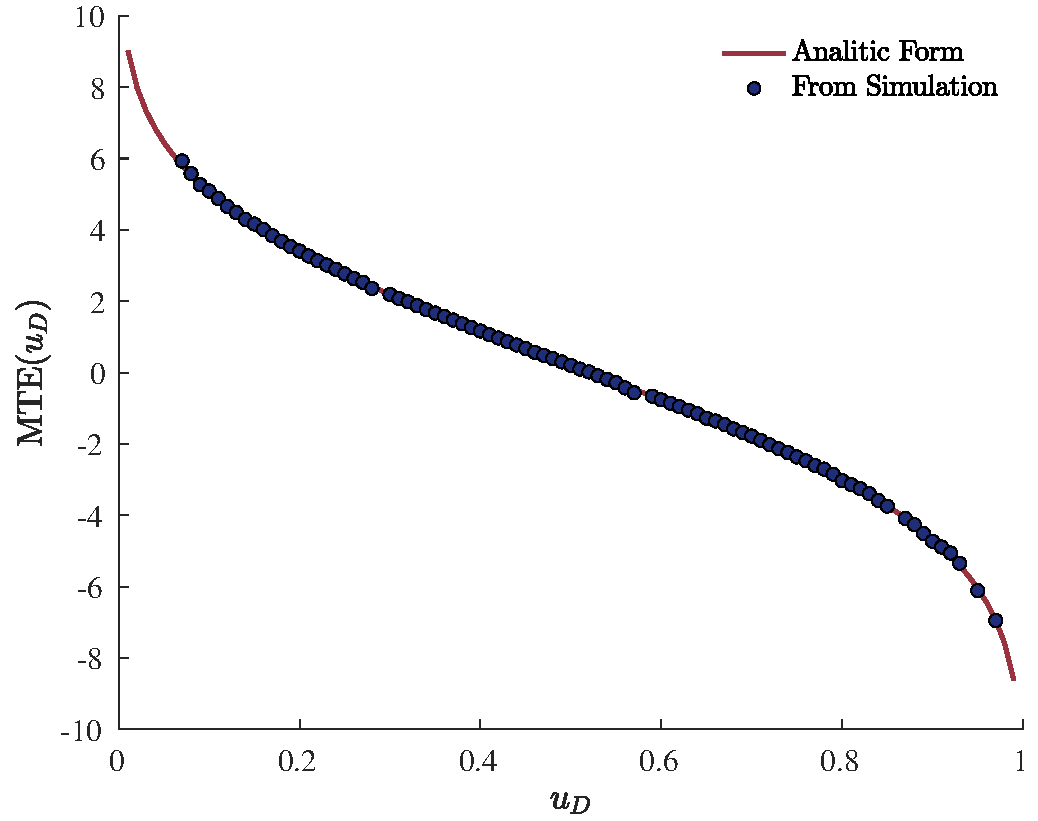
\includegraphics[width=\textwidth]{ps1Heckman/Figures/MTEcompare.pdf}
         \caption{Simulation vs. Analytic}
     \end{subfigure}
     \begin{subfigure}[b]{0.43\textwidth}
         \centering
         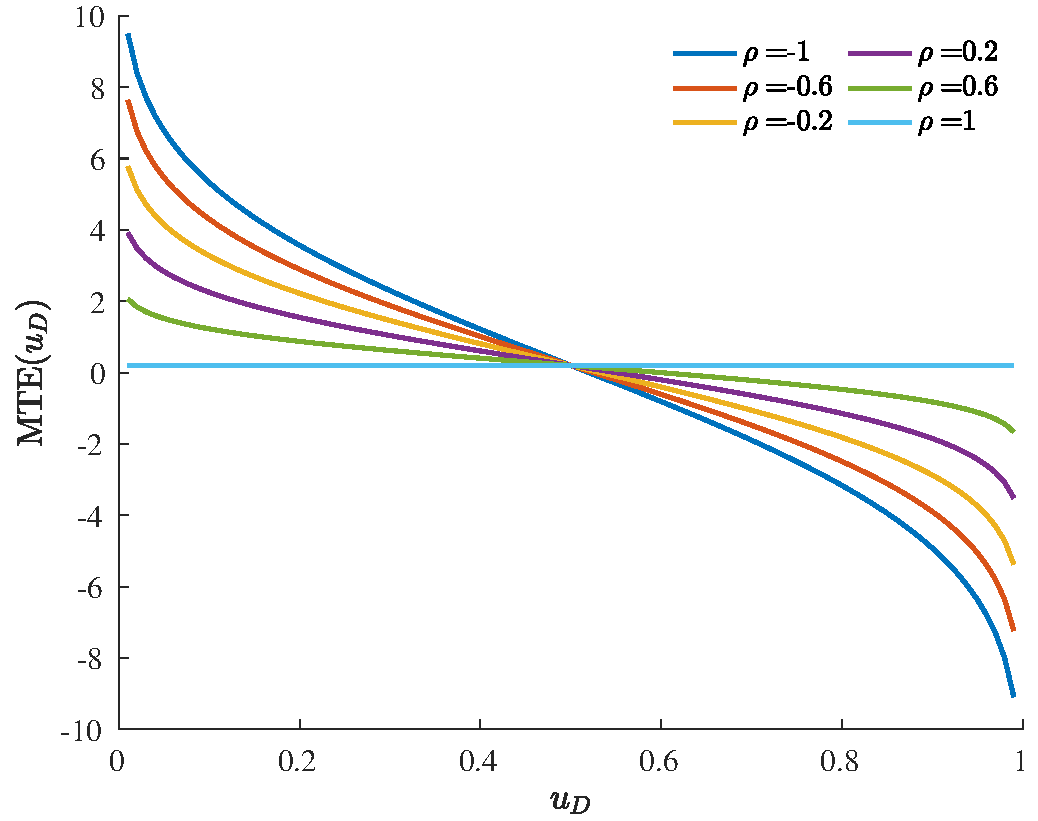
\includegraphics[width=\textwidth]{ps1Heckman/Figures/MTEgrid.pdf}
         \caption{Compare while varying $\rho$}
     \end{subfigure}
\end{figure}
\FloatBarrier
\end{solution}
\begin{problem}{b}
For each case, give LATE for a unit downward change in $C=.5$.
\end{problem}
\begin{solution}
\begin{table}[htb]
\centering
\caption{Treatment effects}
\label{table:te}
\begin{tabular}{lccccc}
\hline
 & ATE & TT & TUT & LATE & PRTE \\
\hline\hline
$\rho=$-1 & 0.20 & 2.70 & -0.66 & 0.98 & 0.98 \\
$\rho=$-0.9 & 0.20 & 2.67 & -0.64 & 0.98 & 0.98 \\
$\rho=$-0.8 & 0.20 & 2.62 & -0.59 & 0.98 & 0.98 \\
$\rho=$-0.7 & 0.20 & 2.59 & -0.56 & 0.98 & 0.98 \\
$\rho=$-0.6 & 0.21 & 2.55 & -0.52 & 0.98 & 0.98 \\
$\rho=$-0.5 & 0.20 & 2.50 & -0.47 & 0.97 & 0.97 \\
$\rho=$-0.4 & 0.19 & 2.45 & -0.44 & 0.98 & 0.98 \\
$\rho=$-0.3 & 0.21 & 2.42 & -0.38 & 0.98 & 0.98 \\
$\rho=$-0.2 & 0.20 & 2.37 & -0.35 & 0.97 & 0.97 \\
$\rho=$-0.1 & 0.20 & 2.32 & -0.30 & 0.97 & 0.97 \\
$\rho=$0 & 0.20 & 2.26 & -0.25 & 0.97 & 0.97 \\
$\rho=$0.1 & 0.20 & 2.22 & -0.20 & 0.97 & 0.97 \\
$\rho=$0.2 & 0.20 & 2.15 & -0.15 & 0.96 & 0.96 \\
$\rho=$0.3 & 0.20 & 2.09 & -0.10 & 0.95 & 0.95 \\
$\rho=$0.4 & 0.20 & 2.04 & -0.05 & 0.95 & 0.95 \\
$\rho=$0.5 & 0.20 & 1.97 & 0.01 & 0.94 & 0.94 \\
$\rho=$0.6 & 0.20 & 1.90 & 0.07 & 0.92 & 0.92 \\
$\rho=$0.7 & 0.20 & 1.82 & 0.12 & 0.90 & 0.90 \\
$\rho=$0.8 & 0.20 & 1.73 & 0.17 & 0.86 & 0.86 \\
$\rho=$0.9 & 0.20 & 1.63 & 0.20 & 0.76 & 0.76 \\
$\rho=$1 & 0.20 & - & 0.20 & - & - \\
\hline
\end{tabular}
\end{table}

\end{solution}
\begin{problem}{c}
What is PRTE for a unit downward change in $C$ ?
\end{problem}
\begin{problem}{d}
Write this model as a random coefficient regression model with $Y=D Y_{1}+(1-D) Y_{0}$ as the dependent variable. $D=1$ corresponds to being in Sector $1 ; D=0$ otherwise. When is least squares a consistent estimator of ATE? TOT?
\end{problem}


\newpage
\section*{Problem 5}
Isaac Newton demonstrated that gravity obeys the following relationship between two objects with masses $m_{1}$ and $m_{2}$ that are $r$ meters apart:
Force: $\quad f=G \frac{m_{1} m_{2}}{r^{2}}$,
where $G$ is a graviational constant. Coulomb later found a similar relationship for electrical charge.
\begin{problem}{a}
Should we discard these laws because they are too functionally formdependent?
\end{problem}
\begin{problem}{b}
 Equation (1) in problem (1) is widely used in economics. For example, Hsieh and Klenow (2009) use it to study misallocation of inputs into manufacturing in India and China. It is a tool in trade in macro and IO. TFP is linked to this model. What is the evidence of Hsieh and Klenow on the validity of the Cobb-Douglas assumption? Does it matter? Should we reject studies based on a Cobb-Douglas function when a large body of evidence supports a CES technology instead?
\end{problem}
\begin{problem}{c}
Show how to test the Cobb-Douglas assumption with data like that
of Hsieh and Klenow (2009). Is their evidence causal?
\end{problem}





\end{document}
